\documentclass[10pt,a4paper]{article}
\usepackage[utf8]{inputenc}
\usepackage{amsmath}
\usepackage{amsfonts}
\usepackage{amssymb}
\usepackage{subcaption}
\usepackage{longtable}
\usepackage[section]{placeins}
\usepackage{graphicx}
\usepackage[numbers]{natbib}
\author{Ignace Bleukx AND Quinten Bruynseraede}
\title{Machine Learning Project: part 1}

\addtolength{\oddsidemargin}{-.875in}
\addtolength{\evensidemargin}{-.875in}
\addtolength{\textwidth}{1.75in}
\begin{document}
\maketitle

\section{Literature Review}
In this first assignment we try to combine basic principles from game theory with the work concerning multi-agent reinforcement learning. Most literature included in this literature review will therefore more of less fall into one of these categories. First we give an overview of the relevant literature, along with their contributions.


\bigskip
\begin{longtable}{|p{5cm}|p{10cm}|}
\hline 
Article & Contribution \\ 
\hline 
\hline
Multi-agent systems: Algorithmic, Game-Theoretic,and Logical Foundations, \citet{mas} & This paper provides a thorough explaination of the different aspect of game theory, including different types of equilibria. These concepts are of importance to us since we will investigate whether or not our learning algorithms converge to one of these equilibria. Furthermore, the paper provides a detailed description of different types of games, such as cooperative games and non-cooperative games, as well as the notion of games in normal form.   \\ 
\hline 
Multi-agent learning dynamics, \citet{phdthesis} &  This thesis on multi agent learning dynamics provides essential information about different game theory aspects. Not all sections are relevant for our initial research on matrix games. Mainly section 2.3 on evolutionary game theory and chapter 3 are relevant. In this last chapter, the replicator dynamics of many matrix games are investigated and explained very clearly. In this chapter we find an example of the learning pattern we would like to observe with our application of different learning algorithms.   \\
\hline 
OpenSpiel: A Framework for Reinforcement Learning in Games, \citet{lanctot2019openspiel} & The paper provides the documentation of the OpenSpiel framework. All aspects of the library are explained, from installation to implemented algorithms and games. Many design choices of the framework are clarified which helps to understand the philosophy behind the framework. In the paper, the game theory aspects are briefly touched upon, as well as important concepts of the implemented learning algorithms. This paper is of very much importance to us as we will use (and potetially extend) the OpenSpiel framework for this assignement. \\ 
\hline  
Reinforcement learning produces dominant strategies for the Iterated Prisoner’s Dilemma, \citet{rlforpd} & 
This document contains a detailed description of the prisoners dilemma. Since this is one of the matrix games we will examine in the first part of the assignement, this belongs to the relevant lecture on this list. Furhermore, some examples of parameters for the training algorithms are given, which will help to produce meaningfull results when training the learning algorithms of choice.\\ 
\hline 
The replicator equation on graphs, \citet{Ohtsuki2006TheRE} & The paper provides an insight on the visualization of the replicator dynamics using phase, as well as some examples relevant to our research. These examples include the prisoners dilemma and biased rock-paper-scissors.\\
\hline
Analyzing Reinforcement Learning algorithmsusing Evolutionary Game Theory, \citet{bloembergenmaster} & This thesis provides a rich source of information on the reinforcement learning branch for evolutionary game theory. Many algorithms are examined, some of which are available in OpenSpiel. The paper also contains the exact parameter settings used to achieve the presented results. These paramters can be used by our agents to reproduce favorable results of the paper. \\
\hline
Evolutionary Dynamics of Multi-Agent Learning:A Survey, \citet{evoldynamics} & Like other papers, this document provides a basic knowledge of game theory, as well as reinforcement learning. For our research, mainly the part about lenient FAQ-learning as a way to increase the robustness of Q-learning, is important. FAQ-learning is able to recover from bad exploration in the start of the run, while normal Q-learning is sometimes not. \\
\hline
Extended Replicator Dynamics as a Key to Reinforcement Learning in Multi-agent Systems, \citet{extrepl} & To model stochastic policies, populations of players are used. These populations can be described using evolutionary concepts, such as selection and mutation. This paper explains the transition from regular to evolutionary game theory. We received insight on the dynamics of a population through the central notion of replicator dynamics. These selection mechanisms can be extended with mutation, based on the Boltzmann mechanism. To overcome converge to suboptimal equilibria, lenience towards mistakes is introduced in this paper.
\\ 
\hline
\end{longtable} 

\section{Independent learning}
%TODO: learn 2 agents on all games, show convergence. Do the learning algorithms converge to Nash equilibria. Are these Pareto optimal?
\section{Dynamics of learning}

\subsection{Lenient Boltzmann Q-Learning dynamics}
Based on \citet{evoldynamics}, we implemented Lenient Boltzmann Q-Learning dynamics. This extension introduces two parameters. The first parameter, $\kappa$, is the degree of leniency: the number of rewards that are examined in each step before updating the policy. We expect to see improved robustness when introducing leniency. Intuitively, this is done by increasing the area of attraction for optimal equilibria. Secondly, $\tau$ introduces entropy into the population: a learner will favour exploration over exploitation when $\tau$ increases. We expect fixed points of the dynamics to stray away from any Nash equilibria as $\tau$ is increased. However, introducing a s small amount of entropy may prevent attraction from unwanted equilibria early on.

\begin{figure}[h]
    \centering
    \begin{subfigure}[b]{0.30\textwidth}
        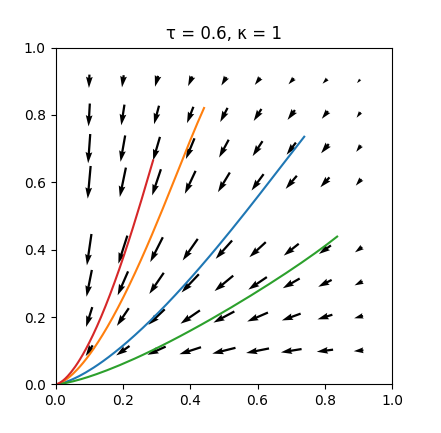
\includegraphics[width=\textwidth]{Figures/boltzmann_pd_1.png}
    \end{subfigure}
    \begin{subfigure}[b]{0.30\textwidth}
        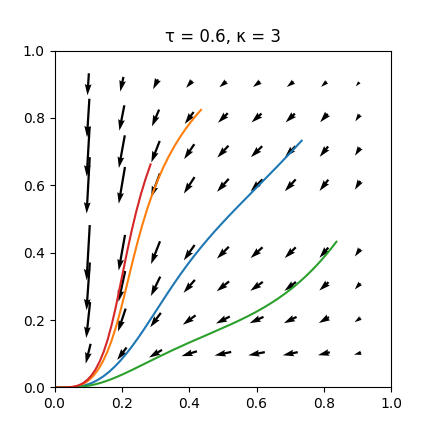
\includegraphics[width=\textwidth]{Figures/boltzmann_pd_3.png}
    \end{subfigure}
    \begin{subfigure}[b]{0.30\textwidth}
        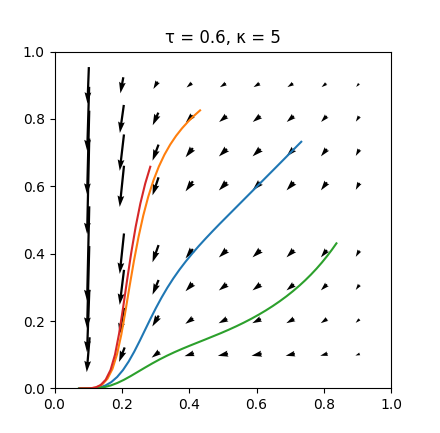
\includegraphics[width=\textwidth]{Figures/boltzmann_pd_5.png}
    \end{subfigure}
    \caption{LFAQ for the Prisoner's dilemma}
    \label{fig:boltz_pd}
\end{figure}

\begin{figure}[h]
    \centering
    \begin{subfigure}[b]{0.30\textwidth}
        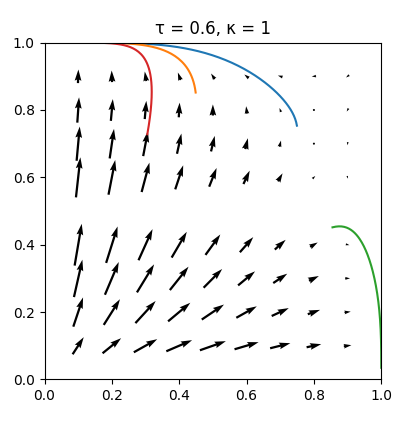
\includegraphics[width=\textwidth]{Figures/boltzmann_bots_1.png}
    \end{subfigure}
    \begin{subfigure}[b]{0.30\textwidth}
        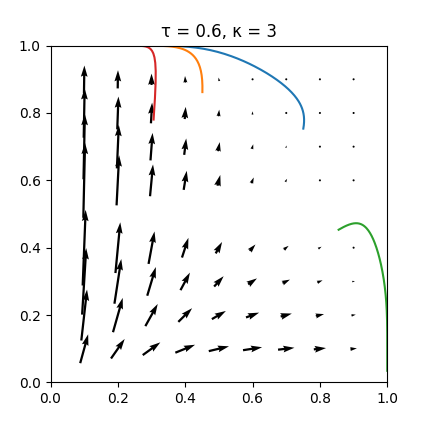
\includegraphics[width=\textwidth]{Figures/boltzmann_bots_3.png}
    \end{subfigure}
    \begin{subfigure}[b]{0.30\textwidth}
        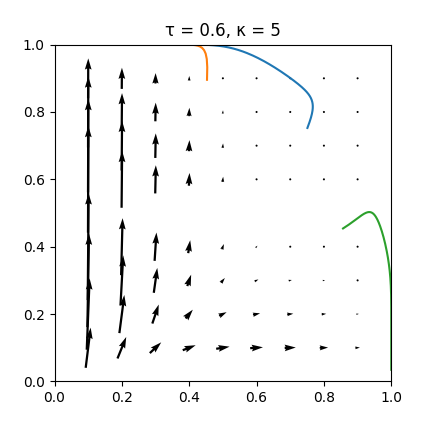
\includegraphics[width=\textwidth]{Figures/boltzmann_bots_5.png}
    \end{subfigure}
    \caption{LFAQ for the Battle of the Sexes}
    \label{fig:boltz_bots}
\end{figure}

\begin{figure}[h]
    \centering
    \begin{subfigure}[b]{0.30\textwidth}
        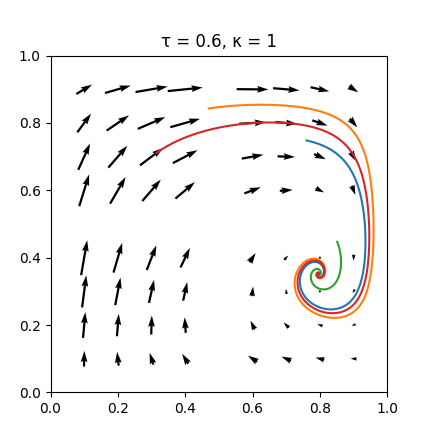
\includegraphics[width=\textwidth]{Figures/boltzmann_mp_1.png}
    \end{subfigure}
    \begin{subfigure}[b]{0.30\textwidth}
        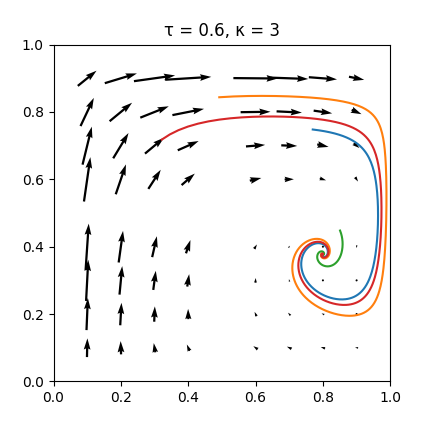
\includegraphics[width=\textwidth]{Figures/boltzmann_mp_3.png}
    \end{subfigure}
    \begin{subfigure}[b]{0.30\textwidth}
        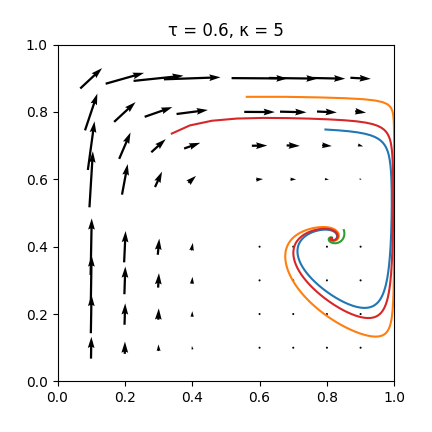
\includegraphics[width=\textwidth]{Figures/boltzmann_mp_5.png}
    \end{subfigure}
    \caption{LFAQ for the Matching Pennies game}
    \label{fig:boltz_mp}
\end{figure}

Figures \ref{fig:boltz_pd} through \ref{fig:boltz_mp} show the influence of the parameter $\kappa$ on the dynamics. For games such as the Prisoner's Dilemma with one equilibrium (in this case located at 0,0), the difference isn't very interesting. However, in Figure \ref{fig:boltz_bots}, we clearly see how there is no longer attraction to the suboptimal equilibrium at ($\frac{2}{5}$,$\frac{3}{5}$).
\\
The influence of $\tau$ is very clear, as shown in Figure \ref{fig:tau}. As $\tau$ increases, exploration of new solutions is greatly preferred. Therefore, an agent will not further capitalize on improvements in his strategy. As a result, policies seem to converge to random guessing.



\begin{figure}[h]
    \centering
    \begin{subfigure}[b]{0.30\textwidth}
        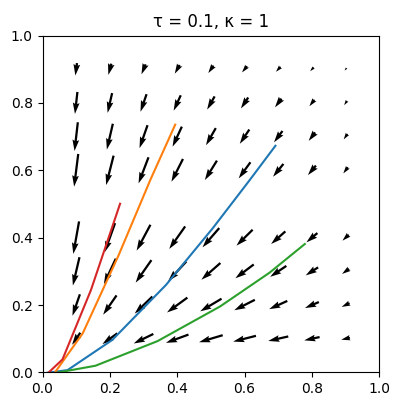
\includegraphics[width=\textwidth]{Figures/boltzmann_pd_temp01.png}
    \end{subfigure}
    \begin{subfigure}[b]{0.30\textwidth}
        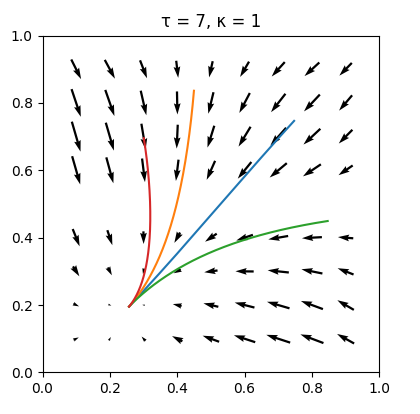
\includegraphics[width=\textwidth]{Figures/boltzmann_pd_temp7.png}
    \end{subfigure}
    \begin{subfigure}[b]{0.30\textwidth}
        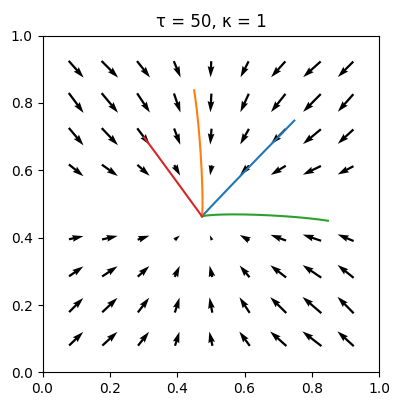
\includegraphics[width=\textwidth]{Figures/boltzmann_pd_temp50.png}
    \end{subfigure}
    \caption{Influence of increasing $\tau$ on the Prisoner's Dilemma}\label{fig:tau}
\end{figure}




\bibliography{lit}{}
\bibliographystyle{plainnat}
\end{document}